% 	Benjamin Van Durme, vandurme@cs.rochester.edu, 24 Aug 2009
%
% Purpose: an example .tex file for the thesis.
%
% This file was derived from those used by Ashwin Lall and Piotr Faliszewski in
% their respective thesis works.

\documentclass[11pt,leqno]{report}

% Feb 24, 2010 vandurme> I used a separate header.tex to capture personal
% shortcuts, and included packages. This allowed my to create mini-documents
% based on each chapter, by having a distinct top-level file around each of the
% files "\include"-ed below, that could each then use the same header (so
% changes would be kept in sync):
%
%\input{header}
%
% The first two things in that header:
%\usepackage{urcsbiblio}
%\usepackage{urcsthesis}

\pdfinfo{
/Title (Extracting Implicit Knowledge from Text)
/Author (Benjamin D. Van Durme)
/Keywords (thesis, knowledge acquisition, information extraction)
}

\begin{document}

\sloppy
\title{Extracting Implicit Knowledge from Text}
\author{Benjamin D. Van Durme}
%\thesissupervisor{Professor Lenhart K. Schubert}
\maketitle

% Feb 24, 2010 vandurme> the graduate office wanted a "ii" on the top right
% corner of the dedication page (lowercase Roman numeral page numbering), which
% explains the slightly messy tex code for this page:

%%%dedication page
\thispagestyle{empty}
%\thispagestyle{plain}
\newenvironment{dedication}
{\cleardoublepage \thispagestyle{empty} \vspace*{\stretch{1}}
  \begin{center} \em}
  {\end{center} \vspace*{\stretch{3}} }
\begin{dedication}

  %% To ... 

\end{dedication}

%%% CV page
%\begin{curriculumvitae}

  Benjamin David Van Durme was born in Dansville, New York on November~13th,
  1979. He began studies at the University of Rochester in 1997, graduating in
  2001 with a Bachelor of Arts degree in the area of Cognitive Science and a
  Bachelor of Science degree in the area of Computer Science. From 2002 to 2004,
  he attended Carnegie Mellon University, and graduated with a Master of Science
  degree in Language Technologies. Benjamin returned to the University of
  Rochester in the Fall of 2004, pursuing research in the subjects of Computer
  Science and Linguistics, under the direction of Professor Lenhart K. Schubert.
  He received the Master of Science degree in Computer Science from the
  University of Rochester in 2006. During the Summer of 2006, as well as 2007,
  Benjamin performed research at Google Inc., under the direction of Marius
  Pa\c{s}ca.

\end{curriculumvitae}

\begin{acknowledgments}

  To my committee as a whole, William Cohen, Gregory Carlson, Daniel Gildea, and
  Lenhart K. Schubert: thank you for your advice and guidance.

  %% Additional personal acknowledgments ...

  Chapter~\ref{ch:Framework} is the result of extensive discussions with Len
  Schubert on a variety of semantic phenomena. Chapter~\ref{ch:Methodology}
  derives from joint work with Len Schubert \cite{vandurmeSTEP08}.
  Chapter~\ref{ch:UsingClasses} is the result of joint work with Ting Qian and
  Len Schubert \cite{vandurmeCOLING08}. Material from
  Chapter~\ref{ch:LearningClasses} is based on collaboration with Marius
  Pa\c{s}ca while at Google Inc. \cite{vandurmeAAAI08}.
  Chapter~\ref{ch:UsingOntology} is based on joint work with Phillip Michalak
  and Len Schubert \cite{vandurmeEACL09}. Chapter~\ref{ch:TopicModels} is based
  on work performed with Dan Gildea \cite{vandurmeTR09}.

  This material is based upon research supported by National Science Foundations
  awards, IIS-0328849 entitled ``Deriving General World Knowledge from Texts by
  Abstraction of Logical Forms'', IIS-0535105 entitled ``Knowledge
  Representation and Reasoning Mechanisms for Explicitly Self-Aware
  Communicative Agents'' and CCF--0910415 entitled ``RI: Small: General
  Knowledge Bootstrapping from Text'', in addition to a University of Rochester
  Provost's Multidisciplinary Award (2008), entitled ``Computational
  Psycholinguistics: Integrating Computational and Behavioral Methods to Study
  Human Language Processing''. Any opinions, findings, and conclusions or
  recommendations expressed in this material are those of the author and do not
  necessarily reflect the views of above named organizations.

\end{acknowledgments}

\begin{abstract}

  The everyday intelligence of both humans and machines relies on a large store
  of background, or common-sense, knowledge. That such a knowledge base is not
  yet available to machines helps partially explain the community's inability to
  provide society with the sort of synthetic intelligence described by futurists
  such as Turing, or Asimov.

  In response, there have emerged a variety of methods for automated
  \emph{Knowledge Acquisition (KA)} that are now being actively explored. Here I
  consider the extraction of knowledge that is conveyed \emph{implicitly}, both
  within everyday texts and queries posed to internet search engines. Through
  recognizing certain forms of existential predicative patterns, and abstracting
  from these to more strongly quantifiable statements, I show that a significant
  amount of general knowledge can be gleaned based on how we talk about the
  world. I provide experimental results both for the direct extraction and
  strengthening of such knowledge, and for the automatic acquisition of
  supporting resources for this task.

  In addition, I draw attention to the relationship between automatically
  acquired background knowledge and natural language \emph{generic} sentences.
  Humans use generics when they wish to directly assert the same sorts of
  ``rules of the world'' that are of concern to the KA community. And yet, there
  has been little recognition in applied circles that decades of work from
  formal linguistic semantics may have a role to play in the representation, and
  perhaps even the acquisition, of common knowledge.
  
\end{abstract}

\tableofcontents
\listoftables
\listoffigures

%Introduction
Commonsense reasoning is the field of artificial intelligence dedicated to simulating and replicating high level intuition in human beings. 
Because many higher level human reasoning processes involve knowledge (intuitive or otherwise) about three-dimensional objects, scenes, and situations, and because significant evidence exists indicating that human minds utilize simulations in three-dimensions when thinking, it follows that reasoning in spatial environments is an intuitive and important part of artificial intelligence \cite{selman1998analogical}. 

Dr. Lenhart Schubert's Epilog project is a natural language processing system which is capable of symbolic reasoning of English utterances. 
The system has shown success in a number of tests, however, does not have a system for reasoning in in three dimensions \cite{schubert2000episodic}. 
Although the system could theoretically reason as such, the act of doing so would require an extensive library of ad-hoc information and costly computation. For example, consider the phrase,

\begin{center} “it is unwise to play leap-frog with a unicorn.” \end{center}

Reasoning about this phrase requires knowledge of the anatomy of both a human and unicorn, the basics of the game leap-frog (i.e. one entity moves from the anterior to posterior of the other, usually passing over the head), and that sharp object cause pain when in contact with certain body parts. 
Rather than hand-code all of these (and more) properties into the system, it makes much more sense to utilize a 3D simulation, where many of these properties are ingrained into the framework.

Luckily, Epilog has a built in framework for integrating so-called “specialists.” 
These programs are additions to the Epilog framework which are able to quickly and efficiently solve logical lemmas over a subset of the overall domain of the larger system \cite{schubert1983determining,schubert1987accelerating,schubert2000episodic}. As a means of supplementing and improving the reasoning capabilities of the Epilog project, and to bring it closer to its goal of accurate simulation of human thought, our group chose to create a specialist for reasoning in three dimensions. 
The project began over the summer and has continued into this year. We have been able to create and implement a system which can successfully place and query entities over a small library of objects and predications.

John McCarthy was the first to formally identify the concept of commonsense reasoning in literature, and described it as 

\begin{center}
 ``the ability of an agent to deduce a sufficiently wide class of immediate consequences of anything if it is told what it already knows'' \cite{mccarthy1963programs}.
\end{center}
  
For his seminal Comirit project, Dr. Benjamin Johnston completely rejected any definition of common sense period \cite{johnston2008comirit}. 
Over the course of all surveyed literature, there are a number of consistencies in the various definitions (both implicit and explicit) of commonsense reasoning in artificial intelligence. 
Some common themes are:
\begin{center}
\begin{enumerate}
	\item The ability to quickly reason on a series of mundane topics and issues
	
	\item Deduction capabilities on high-level, well known topics to which the system has been exposed previously
	
	\item knowledge of a wide variety of topics and of relationships and interactions of entities within
	
	\item an emphasis on rapidity of reasoning rather than accuracy or precision
\end{enumerate}
\end{center}

The use of symbolic logic is also worth noting in the field of commonsense reasoning. Symbolic reasoning has been an integral part of a number of programs meant to emulate common sense. Dr Johnston's Comirit utilizes a tableaux reasoning which uses proof by resolution in conjunctive normal form propositional logic in order to make logical deductions \cite{johnston2008comirit,johnston2009practical}. the Soar project also utilizes a symbolic logic processing unit in addition to it 3D simulations in a very similar manner \cite{wintermute2009overview}. McCarthy's original advice-taker and advice-giver programs were entirely symbolic, relying on forward inference in order to make deductions and reach conclusions based on the given data in its knowledge base and input from the user \cite{mccarthy1963programs}.
Although statistical methods could potentially be used in this field of AI, the vast majority of literature utilizes symbolic or logical methods.

\section{Commonsense Problem Formulation}
Commonsense reasoning problems are approached from a different perspective from that of other AI problems. While many AI agents attempt to create an agent that can efficiently execute one task that supposedly requires ``intelligence,'' commonsense reasoning problems are broader, and less deal with a less precise form of knowledge. For this reason, commonsense problems are often solved with general solutions with less precise metrics than other problems \cite{johnston2008comirit,johnston2009practical}.

One of the first commonsense problems was the ``Tweety problem.'' This involved a human feeding a story into an AI agent; this story progressively described an entity ``Tweety.'' It was proposed that an agent with common sense would be able to infer that Tweety was a bird, and thus infer that it could likely fly. The agent would also be able to adjust it's mental preception of the bird, perhaps inferring it to be a flightless bird, such as a penguin, if it was later stated that Tweety could not fly \cite{johnston2008comirit,egg-cracking}. This problem requires a broad thinking over the general properties of a number of topics and objects, and the inference process is inexact and nebulous.

The ``egg-cracking'' problem is also one of the more famous lemmas of commonsense reasoning. In this problem, as with the Tweety problem, an agent reads a story about a chef making a cake (one of the steps of which is cracking an egg on the bowl and pouring the contents inside). The agent is then asked a series of questions about the scenario. These interrogations usually have a broad range, but would be considered trivial to a human (``why doesn't the chef throw the whole egg into the bowl?'' ``What will happen if the chef does all the motions very slowly?'') \cite{egg-cracking}. In sum, the primary features of commonsense benchmark problems can be summarized in the following points:
\begin{center}
	\begin{itemize}
		\item open problem domains
		\item evaluation based on the answering of na\"{i}ve questions
		\item focus on ``breadth'' knowledge, rather than ``depth''
	\end{itemize}
\end{center}

\section{Significance}
The importance of a system to reason in common sense is readily apparent to the non-technical thinker. 
Nearly every task a human undertakes requires an implicit knowledge of everyday commonsense, and as such, the field of reasoning is almost inseparable from most of the end goals intelligent artificial agents \cite{johnston2009practical, johnston2008comirit}. 
Tasks such as navigating a road during rush hour and pouring wine into a glass properly require naive knowledge of a variety of topics, such as traffic etiquette, physical properties of liquids and solids, acceleration and deceleration of automobiles, etc. There is also a suprising robust amount of existing data for commonsense systems. Johnston cites that many video games implement commonsense reasoning in the form of enemy AI \cite{johnston2008comirit}. Further, common sense is, by definition, possessed by a large percentage of the human population. Because of this, there is a very large potential workforce for compiling or otherwise working with common sense reasoning systems. This has already been implemented with an online application for creating common 3D figures \cite{johnston2011collection}.

The generality of commonsense reasoning is one of its primary benifits. Almost any real world problem will have to deal with an open domain. It is clear that the world does not operate on anything even approximating the extremely controlled and limited worlds commonly evaluated in most computer environments. If an AI agent is to solve real-world problems, it must be able to solve more than a very narrow range of problems, and deal with the numerous contingencies that arise in real world scenarios. \cite{egg-cracking,johnston2009practical,johnston2008comirit,schubert2000episodic,mccarthy1963programs}.

\section{3D Simulations}
Hand in hand with commonsense reasoning is the role of 3D simulations. 
In an informal sense, a simulation is the ability to construct (or in some cases, reconstruct) physical scenes from symbolic data. 
More formally, a simulation is a type of analogous representation which begins with a description of a system which changes based on a causal description of the system \cite{gardin1989analogical}. Simulations have been used many times in the course of both AI and cognitive science. McCarthy first suggested using simulation in his ``advice taker'' program. Since then, the concept has reappeared many times in literature. In particular, physical systems (those representing real-life physics) have implemented with simulation.

 Previous examples of this in Gardin et al's use of “atomic spheres” to model liquids and their properties. This example implements spherical objects (analogous to atoms) which behave collectively as a liquid. The simulation of gravity along with these structures enabled a primitive AI to learn to correctly fill a glass. Johnston was able to accomplish a the same results with Comirit's \cite{gardin1989analogical,johnston2008comirit}. The Soar project also implemented 3D simulations; by creating a 3D environment and testing object positions within, the system was able to deduce rudimentary physical properties and solve related problems \cite{wintermute2009overview}.

The relation between 3D simulations and commonsense reasoning is apparent. As mentioned earlier, commonsense reasoning's primary domain is real-life situations. Human beings are creatures who live in a environment with three spatial dimensions and one time dimension, physical laws are well defined and inescapable in the real world. This means that the most apparent and relevant environment for solving commonsense lemmas is one which incorporates the properties and aspects of the real world \cite{johnston2008comirit,johnston2009practical}.

Cognitive science has observed that humans process their physical environments as a series of simulations: forming an initial mental image and adjusting it over time in order to deduce properties about it \cite{gardin1989analogical}. 
Thus, there is considerable evidence and motivation for utilizing simulations in AI, particularly in a program designed to model and reason in physical situations.
The implementation of such a system as a specialist in the Epilog system also meshes well with previous experiments and evidence.

The incredibly complex spatial situations of three-dimensional simulations are far to computationally intense and convoluted for a symbolic logic system to represent by itself. 
The aid of a specialist provides a more narrow computational domain which can soundly and quickly compute responses to queries over a sub-domain of problems (in our case, problems pertaining to reasoning in spatial environments).

\section{Specialist Programs}
The usage of specialist programs (as opposed to stand alone programs) has shown to be an effective means of programming common sense. While many programs exist as single-component entities, a large proportion of AI programs, as mentioned earlier, deal with a much narrower scope than commonsense reasoning problems \cite{johnston2008comirit,johnston2009practical}. Because of this, there is less of a need for specialist programs because the entire program is a specialist. However, commonsense reasoning requires breadth, not depth, and thus encounters the problems predicted by the clich\`{e}, though true, axiom of software engineering, and life in general: one cannot be good at everything.

Resolution theory provides a formal justification for specialist programs. The central premise of this is that if a given set of clauses each contains a set of sub-clauses which are mutually incompatible (contradictory), then at least one of those clauses need not be true. This allows a considerable narrowing down of the state space needed in order to solve a problem. Because of this, mutual incompatibility of logical atoms are essential to specialist construction. Schubert et al successfully implemented specialists for Epilog for time, color, and part relationships \cite{schubert1983determining,schubert1987accelerating,schubert2000episodic}. 

Thus, commonsense programs will likely need to be broken down into functional units. One of these units would specialize in 3D spatial reasoning. As mentioned above, it is infeasible and awkward to compute problems relating to 3D space in a purely symbolic environment. These computations, however, are very necessary for a true commonsense reasoning system. This lays the foundation for the motivation for the \TDS project. 

\section{Usage in the \TDS and Connection to Epilog}
The Epilog Project is a natural language processing program which seeks to implement commonsense natural language understanding. The system is distinct from other, more traditional means of representing natural languages formally (such as first-order logic) in that it allows for complex and rich concepts such as belief systems, and, as the name of the system suggests, explicit references to time frames. It is from this feature that the name Epilog (EPIsodic LOGic) is derived \cite{schubert2000episodic}.

It is apparent as to how this focus on time frames is closely related to simulation. Just as simulation environments involve updating scenes according to a set of defined rules and relationships as the passage of time occurs, Episodic Logic seeks to divide the world into distinct moments in time and create a logical framework from this \cite{selman1998analogical,schubert2000episodic}.

Epilog does not, however, contain methods for accurately or quickly evaluating stories that exist in 3D environments, nor use knowledge based in this frame of reference. Epilog also has a well defined interface for creating and connecting specialist programs to the larger program. This high level of modularity means that specialist programs can be created easily for the greater Epilog project \cite{schubert2000episodic}. The best solutions is, therefore, to utilize the ``time-slice'' centric approach of Episodic logic, as well as the existing specialist interface, and construct a specialist for reasoning in 3D environments.

In keeping with the established paradigm for commonsense program evaluation, it is most appropriate to base the evaluation of the specialist with a test of a broad range of knowledge that operates at a level that is considered ``simplistic'' by human standards. For this reason, childrens' stories provide an excellent source. The following passage, taken from from Lesson 32, Harris et al. 1889, provides information on a visually rich scene, one which requires a wide range of knowledge of spatial relations and laws in order to understand correctly:

\begin{center}
	\begin{enumerate}[topsep=0pt,itemsep=-1em]
		\item Oh, Rosy! Do you see that nest in the apple tree?
		\item Yes, yes, Frank; I do see it.
		\item Has the nest eggs in it, Frank?
		\item I think it has, Rosy.
		\item I will get into the tree.
		\item Then I can peep into the nest.
		\item Here I am, in the tree.
		\item Now I can see the eggs in the nest.
		\item Shall I get the nest for you, Rosy?
		\item No, no, Frank! Do not get the nest.
		\item Do not get it, I beg you.
		\item Please let me get into the tree, too.
		\item Well, Rosy, here is my hand.
		\item Now! Up, up you go, into the tree.
		\item Peep into the nest and see the eggs.
		\item Oh, Frank! I see them!
		\item The pretty, pretty little eggs!
		\item Now, Frank, let us go.
	\end{enumerate}
\end{center}

This story covers a number of physical scenarios and implicit information that can only be deduced with a sufficient understanding of the spatial laws of nature. For example, a specialist should be able to simulate a tree, two children (Rosie and Frank) the nest in the tree, and the fact that the eggs in the nest are visible from above the nest, but not below. This presents a broad knowledge scenario which tests the abilities of an agent to reason in an open-ended, commonsense environment. This is consistent with the evaluation methods for previous entries in literature, and as such is a good metric for the \TDS \cite{egg-cracking,johnston2008comirit,schubert2000episodic}. For the demonstrative purposes of this project, the 3D Specialist should be able to do the following:

\begin{center}
	\begin{enumerate}
		\item construct a scene where
		\begin{itemize}
			\item a person is under a tree
			\item a nest is in a tree
			\item an egg is in the nest
			\item the person can see the nest
		\end{itemize}
		\item deduce that the person can see the nest (though the vision may be obscured by branches)
		\item deduce that the person cannot see the egg (because the nest is in the way)
	\end{enumerate}
\end{center}

This scenario provides a diverse assortment of predications, objects, and conjectures about the story, such that the above tasks will be an important indication of whether or not the system is capable of larger, more complex inferences in commonsense reasoning.

\section{Object Construction and Placement}
From the more concrete aspect of 3D simulation, the methods by which objects are modeled in the 3D scene, and the methods by which they are placed to satisfy logical constraints, are a matter of considerable importance.

Most of the simulation work surveyed constructs objects in a very similar fashion. 3D object made of polygons bound together are the norm for 3D simulation \cite{xu2002constraint,wintermute2009overview,wordseye}. Further, there is a plethora of existing software that utilizes this ``face, mesh, vertex'' paradigm. Thus it makes the most sense to utilize this model in order to capitalize on the fruits of previous research.

Both Soar, Wordseye, and CAPS utilized similar placement methods for objects. Soar utilized the concept of ``legal areas:'' distinct areas of three-dimensional space that represented potential locations for object placement that satisfied predications \cite{wintermute2009overview}. Similarly, the CAPS project implemented ``legal polygons,'' the two dimensional equivalent \cite{xu2002constraint}. Wordseye uses a combination of the two: both three-dimensional placement areas and two-dimensional legal polygons, as a means of specifying areas where object can be placed in order to satisfy predications. In addition, Wordseye also object ``tagging,'' labeling certain parts of objects as relevant areas for certain predications, as a means to aid in object placement. For example, the hand of a person model is tagged with as being able to hold certain objects. If the scene requires the person to be holding an apple, the area specified by this tag becomes the critical point.       
                         
\include{framework}        

The Blender software (www.blender.org) was chosen as the simulation environment for our project.
Blender is a free, open source program designed for 3D modeling, physics simulation, and game design. 
Blender provides a means of easily creating 3D objects, attaching properties and constraints to those objects, and developing scripts that interact with the software and objects.

Models in Blender are stored as ``objects'' with associated ``meshes.'' 
A mesh is a data structure with a series of faces, edges, and vertex locations in space for the object. 
Blender also contains methods for adding custom properties to objects, which serves to make the system quite extensible.
Native support for 3D modeling and operations is highly desirable as well. 2D approaches were also considered, but possessed limited support for modeling and manipulating scenes in 3D. 
With Blender's existing 3D support and extensive library utilities for 3D object management, the task of developing a simulation environment is eased considerably.

Blender contains a very accessible Python API. 
This allows Python scripts to access methods in Blender, and allows the system to create and change objects, measure properties of these objects, and even instantiate physical laws (such as gravity) in the scene. 
The direct purpose of this system is to allow Epilog to communicate with a built in series of Python scripts, which then, in turn, will utilize Blender to construct a 3D environment, which can then be examined to derive information about the scene to be fed back as input into Epilog. 
These functions are to be performed incrementally, i.e., in support of a sentence-by-sentence story understanding process. 

The \TDS exists as a series of Python files and a database of objects which interface with Blender. Please note that, from this point on, direct references to structures in the code will be indicated by \texttt{courier} font.

\section{High Level Overview}

The source folder contains three Python files: 
\begin{enumerate}
	\item \texttt{Classes.py}
	\item \texttt{predMethods.py}
	\item \texttt{obutils.py}
\end{enumerate}
A single directory, \texttt{ObjectData}, is also included.

\texttt{Classes.py} file is the highest level Python file, and serves as the top level of the system's organization and control. \texttt{Classes.py} contains three classes: 

\begin{enumerate}
	\item \texttt{Scene} 
	\item \texttt{Entity}
	\item \texttt{Predication} 
\end{enumerate}
	
The \texttt{Scene} class serves to hold the information currently being modeled in the Blender scene, to provide methods for adding entities and predications to the scene, and for querying the scene for how well a given predication is satisfied. 
Although object placement in the system is meant to ensure that all the predications in a given scene are satisfied, this is not necessarily the case. The predications may very well be mutually unsatisfiable, and in keeping with the central purpose of this project, a quick and slightly less accurate placement mechanism is preferable to a more accurate, but much slower one.

Each instantiation of the \texttt{Entity} class stands for an entity in the domain of the scene being modeled. 
An entity is any object in the scene which can be modeled as a Blender mesh object.
The \texttt{Entity} class contains attributes for storing information about the given entity - including a pointer to the object being modeled in the Blender scene - and methods for interacting with the object in the Blender scene.
	
Each instantiation of the \texttt{Predication} class is a predication active in the current scene. 
A \texttt{Predication} instance contains references to the Blender [parent] objects bound by the given predication, and a method for returning placement constraints for either of the objects relative to the other, and one for querying how well the predication is satisfied given the current locations/orientations of the \texttt{Predication}'s objects in the Blender scene. 
The \texttt{Predication} class is generic, and imports placement and querying methods specific to a given predication (e.g. ``near'', ``above'') from the \texttt{Classes.py} file. 

Note that the actual functions for the predication are stored as variables in each class instantiation. 
Once the methods are copied from \texttt{predMethods.py}, \texttt{predMethods.py} is no longer called directly by the predication.

\texttt{predMethods.py} contains placement and query methods for each predicate, for example (respectively) \texttt{nearP} and \texttt{nearQ} for the ``near'' predicate. 
Many of these predicates involve complex functions in Blender's three-dimensional space, which are stored in \texttt{obutily.py}.
\texttt{obutily.py} consists of various methods for operating on Blender objects, and is used by both \texttt{predMethods.py} and \texttt{predMethods.py}.
The full table of the methods for \texttt{predMethods.py} and \texttt{obutils.py} can be viewed in final section.
This ontology was chosen because of how well it fit in with existing Epilog framework. Epilog's internal ontology already defines the domain of discourse into subcategories denoting objects, events, predications, etc. \cite{schubert2000episodic}. Thus, it makes sense to partition the \TDS's ontology similarly. Entities (individuals existing in real space) and predications acting on these entities are explicitly defined in the current model. The other relevant features of the scenes, such as episodes, are built into the framework of the system. For example, an episode is defined as the current arrangement of objects and predications at a given moment within the simulation. This utilizes the built-in model of the \TDS as a specialist is utilized.

\section{Objects and Entities}

The ObjectDatabase directory contains two sub-directories: 

\begin{enumerate}
	\item OBJ 
	\item XML
\end{enumerate}
 
These correspond, respectively, to the two types of information being stored for each object: the three-dimensional model of the object as used by Blender, and other information about the object that is not directly used by Blender. 

In the \TDS, entities are modeled in Blender not with a single mesh, but with separate meshes corresponding to each of the entity's parts. 
When an entity's meshes are imported to the scene, the \texttt{Entity} class imports entity \textless .obj \textgreater-format object files from the \textless item name \textgreater subdirectory in the OBJ directory, where ``item name'' stands for the entity's key (e.g. ``person'' or ``house''). In the Blender scene, these part meshes are bound as children under an empty-point Blender object that is the parent. In the \texttt{Entity} class, the pointer to the Blender object is a pointer to this empty parent object (from which children/parts are easily accessed). Figure \ref{fig:mirs_flow} illustrates the flow of information and interaction between components.

\begin{figure}[h]
	\begin{center}
		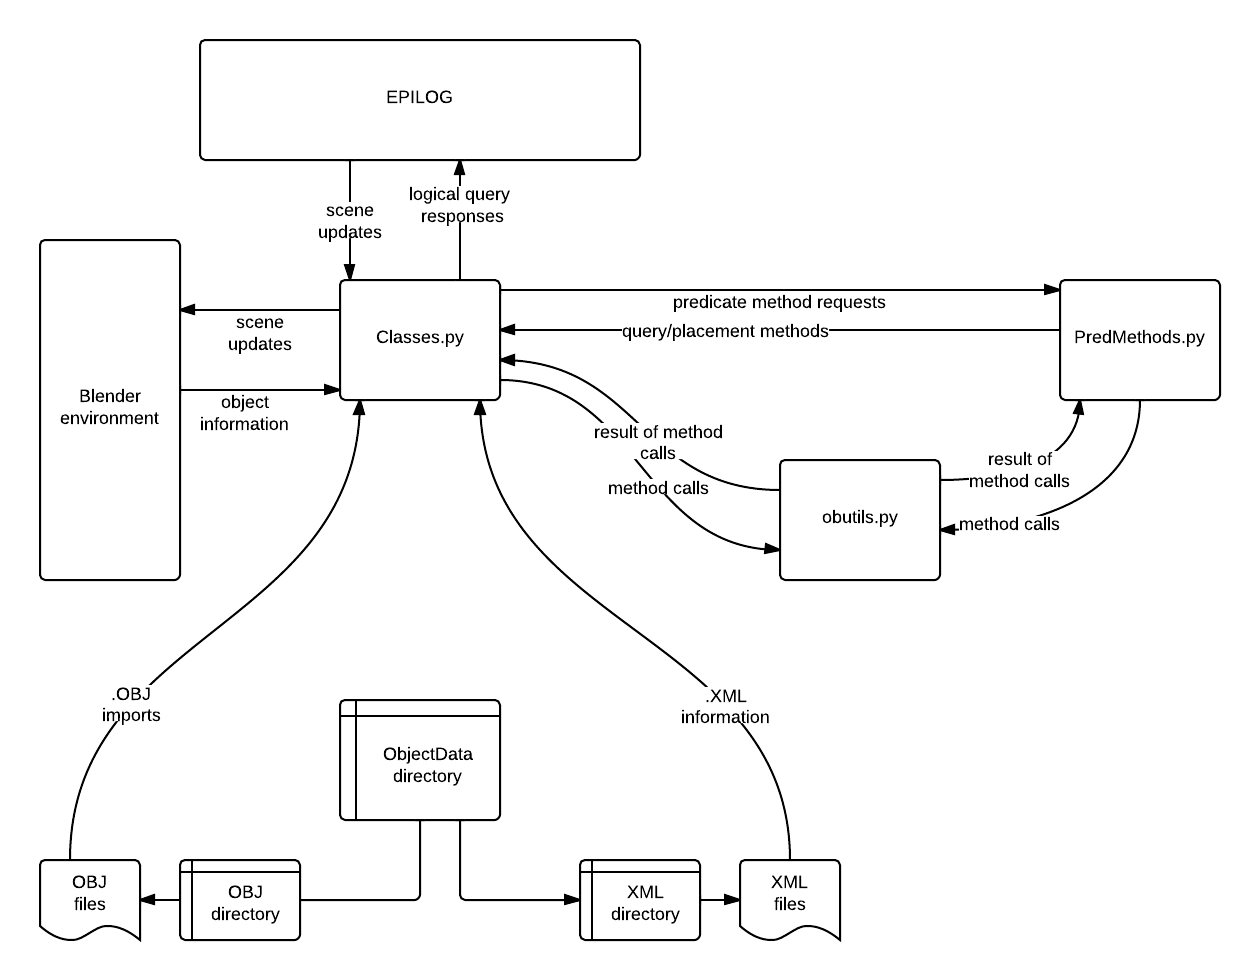
\includegraphics[width=1\textwidth]{figures/mirs_flow.png}
		\caption{The basic flow of information in the \TDS.}
		\label{fig:mirs_flow}
	\end{center}
\end{figure}

The XML directory contains \texttt{\textless item name\textgreater.xml} files for each entity for which there exist Blender models, where \texttt{\textless item name\textgreater} \xspace stands for the entity's key. Each XML file contains the following information: a meronomy graph for the entity, a list of the parts with meshes, and finally bounding box coordinates for the object. 
Periodic updates, predominantly introduction of new objects and predications, as well as changes to existing objects and predications, are sent to the specialist by Epilog.

Although a very extensible sotware system, Blender was not designed specifically for the complex scripting that this project utilized. As such, several object and code issues were encountered with the Blender system that needed to be documented.
First, many of the objects in the system did not have \emph{well-formed} meshes. 
\emph{Well-formed} in this case has very specific meaning. 
In this case, a blender mesh is said to be \emph{well-formed} if it contains closed objects with no holes in the mesh, edge loops (which define faces) which are connected and form a closed loop, and no disconnected components. 
Unfortunately, several objects in the system (notably the “chair” object) contain some glitch in their meshes which renders them not \emph{well-formed}. 
This can cause several errors when intersection and difference algorithms (or other methods which involve mesh operations) are utilized by the system.
These changes were made, and the objects were able to function correctly.

There are further limiting factors that were noted when utilizing Blender to place and measure objects. Due to the algorithms used in the volume calculation:

\begin{center}
	\begin{itemize}
		\item Faces and Edges cannot be placed directly on top of one another, an offset (even as small as 0.001 BU) of one of the objects must be used
		\item Even if an object is deleted from Blender's scene environment, it's mesh information will still remain. This can slow down the computation of built-in functions in blender whose run-time scales with the total number of meshes in the scene. As such, scenes must be restarted for multiple rounds of testing to ensure accurate, releiable data.
	\end{itemize}
\end{center}

\section{Predications}
My particular work has focused on the construction of the predicate class, as well as the helper methods in \texttt{obutily.py}, and management and organization of the program files.
Each \texttt{Predication} instance contains two methods: \texttt{Place()} and \texttt{Query()}. These predicates are stored as \texttt{\textless predicate name\textgreater P} and \texttt{\textless predicate name\textgreater Q}. 
As shown above, the placement function of the near predication is \texttt{nearP} and the query function is \texttt{nearQ}. Query methods evaluate the scene and return a value for how well the given predicate is satisfied in the current scene. 
This can be done continuously as a value between 0.0 and 1.0, or as a boolean. 
For a boolean value, the continuous answer is still evaluated: 1.0 is returned if the answer is above 0.5, and 0.0 if below.
The purpose of the \texttt{BinaryFlag} attribute in the \texttt{Predication} class is to determine whether the predicate is evaluated as a boolean value or not.



\subsection{Vision Predication}
By far, the largest and most complicated predicate was \texttt{canSee(A,B)}.
The implementation of this function relied heavily on ray-casting and went through several iterations before a sufficient model and algorithm were developed. 
The querying method for this predication originally was to be implemented as a single ray-cast, from one object's center to another.

A number of different attempts to construct a sufficient \texttt{canSee(A,B)} function were tested, yet none were of the quality needed for the project. Examples include the use of a conical object expanding from entity A's ``eye'' to B and noting the percent of B's volume that was encompassed inside. Several functions in Blender's Game Engine were also implemented. Early on, a function existed which ray-casted from the center-point of A to the center point of B. This function was naively simple, but proved itself to be surprisingly difficult to implement. For a graphical representation, Figure \ref{fig:vision1} below illustrates the ideal for this model. Note that in this (and future) diagrams, a solid line represents the actual ray cast, and a dotted line represents the remainder distance that the cast would have traveled if there had not been an object in the way acting as an interrupting agent.	
	
\begin{figure}[h]
	\begin{center}
		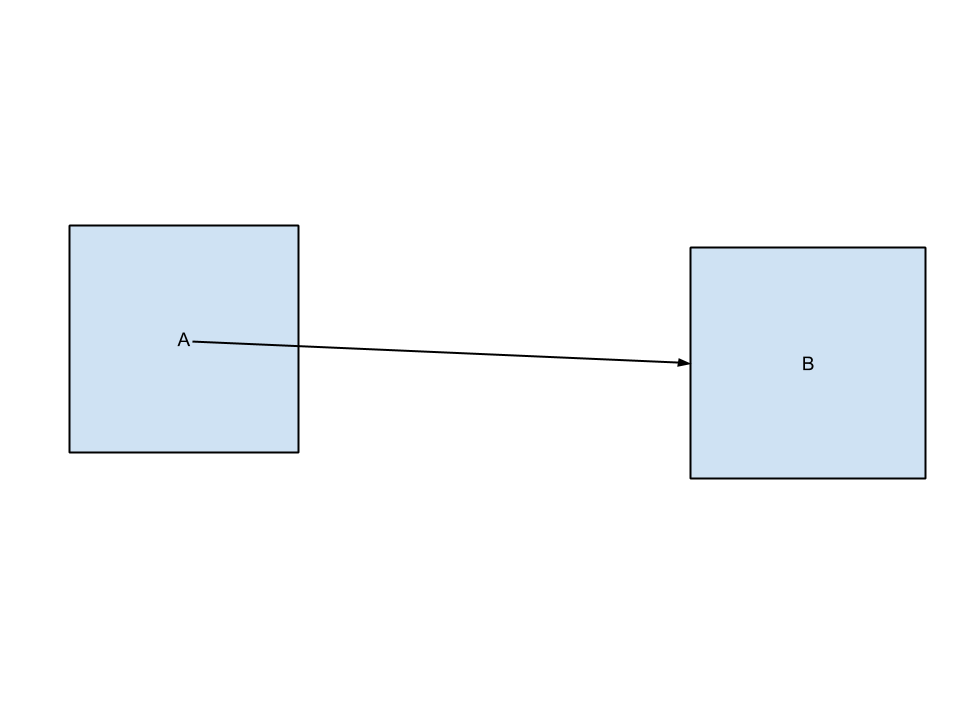
\includegraphics[width=0.48\textwidth]{figures/vision1.png}
	\end{center}
	\caption{an idealized model of the naive implementation of \texttt{canSee(A,B)}.}
	\label{fig:vision1}
\end{figure}

One issue that came up with this design was the collision nature of ray-casting. Namely, a given ray-cast in Blender will return when it hits an object, any object. This means that casts from A's center would always stop upon hitting A's outer mesh. One early attempt to solve this was to simply implement repeated casting: the method would cast continuous rays from the end of one to the start of the other until the end object was met. Figure \ref{fig:vision2} shows the idealized version of the function of this implementation of the function.

\begin{figure}[h]
	\begin{center}
		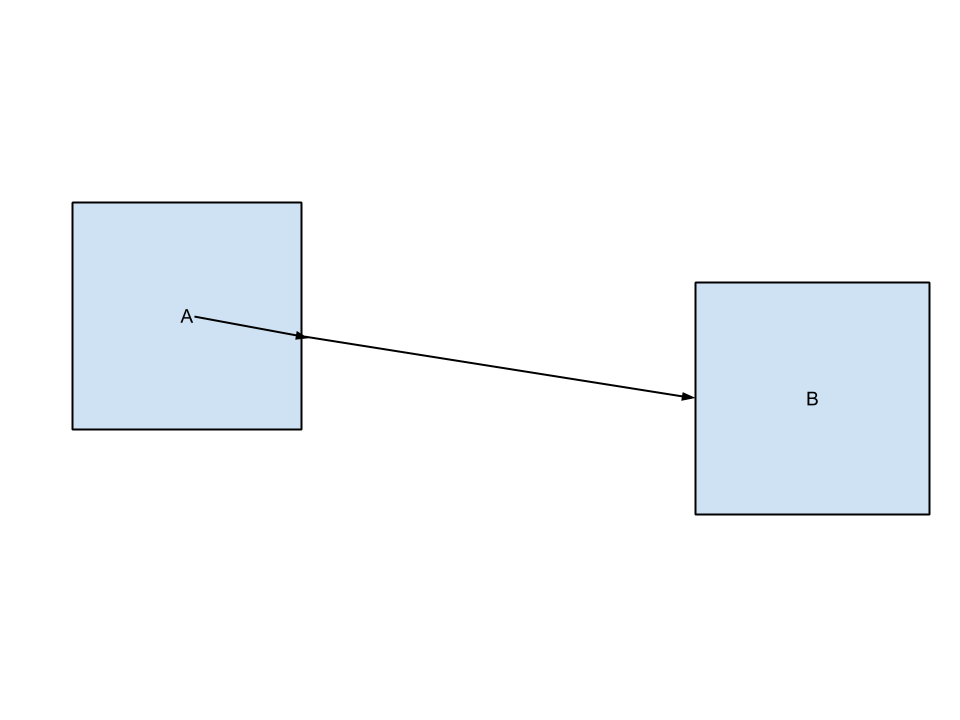
\includegraphics[width=0.48\textwidth]{figures/vision2.png}
	\end{center}
	\caption{A second implementation of ray-casting}
	\label{fig:vision2}
\end{figure}

This revealed yet another problem, however, as casting from the face of one object (which was the collision point of the fist ray-cast in the above) would simply return the starting point of the cast. The ray-cast could repeat infinite times and still be stuck on the same point. The third iteration of this function was meant to fix this. This iteration involved the addition of another method in \texttt{obutily.py}, \texttt{nudge}, which would return an infinitesimally small distance closer to the end point. This function allowed repeated ray-casting to continue unabated and as planned. The new model for ray-casting in this simple iteration is illustrated in figure \ref{fig:vision3}. 

\begin{figure}[h]
	\begin{center}
		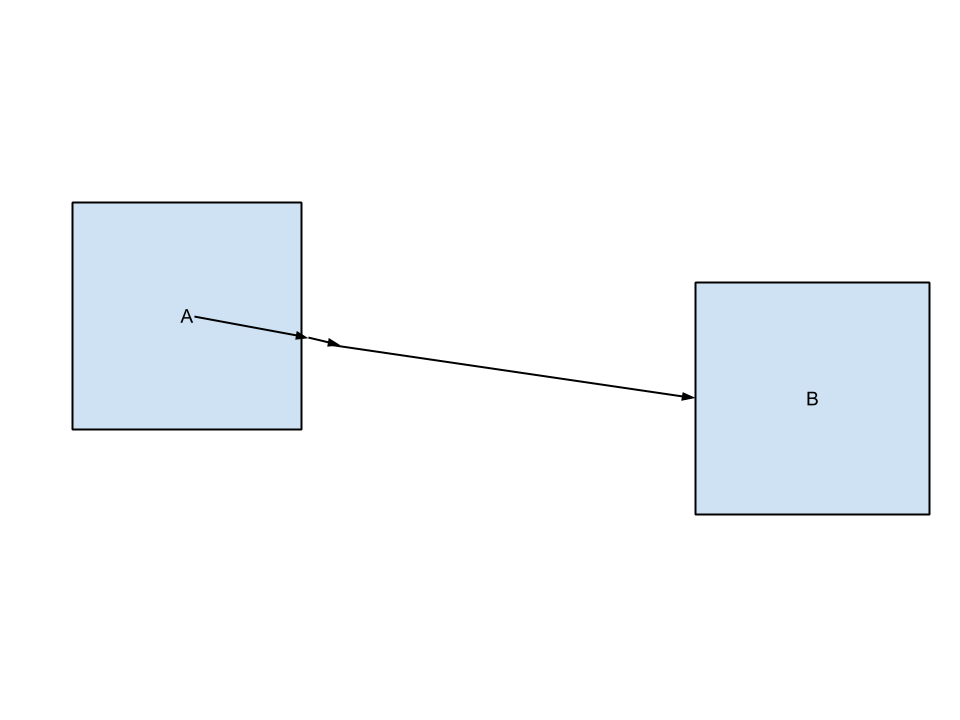
\includegraphics[width=0.48\textwidth]{figures/vision3.png}
	\end{center}
	\caption{The nudge addition to the naive model}
	\label{fig:vision3}
\end{figure}

This model was able to accurately cast a ray from the center of A to B, stopping when it hit B's outer mesh. However, the naive model was, as the name should suggest, not sufficient and could easily return erroneous answers. For example, if there was an object in between A and B which could block the cast, then the method would conclude that A could not see B, even if it were obvious that a line of sight existed between the two. Figure \ref{fig:vision4} illustrates this.

\begin{figure}[h]
	\begin{center}
		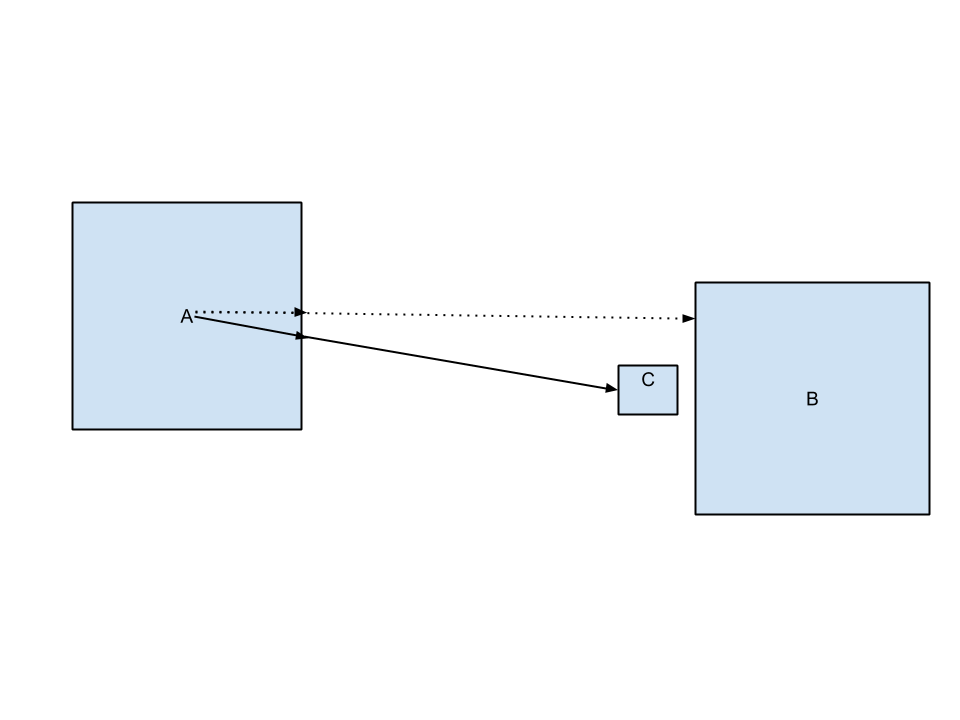
\includegraphics[width=0.48\textwidth]{figures/vision4.png}
	\end{center}
	\caption{C blocks the site of A, even though there exist obvious casts (dashed) that would indicate that B is visible}
	\label{fig:vision4}
\end{figure}

It was obvious early on that this implementation would only serve as a template for future endeavors.
The second model cast a slew of rays from A to the vertices of B. This improved over the naive implementation in two ways. First, it allowed a varying degrees of visibility. Several of the rays may reach their target, and several may not, which allowed for a sense of “partial obscurity” which was not allowed in the original model. This ran into a small technical issue early on, however, as rays would not return if they made contact with the vertices of an object. Due to a technicality in Blender, casts would only return if they made contact with the face of an object. As such, a modification of the nudge function was implemented which pushed the end point of the casts closer to the center. This way, there was a guarantee that the casts, if unobstructed, would hit the object properly. Figure \ref{fig:vision5} illustrates this model.

\begin{figure}[h]
	\begin{center}
		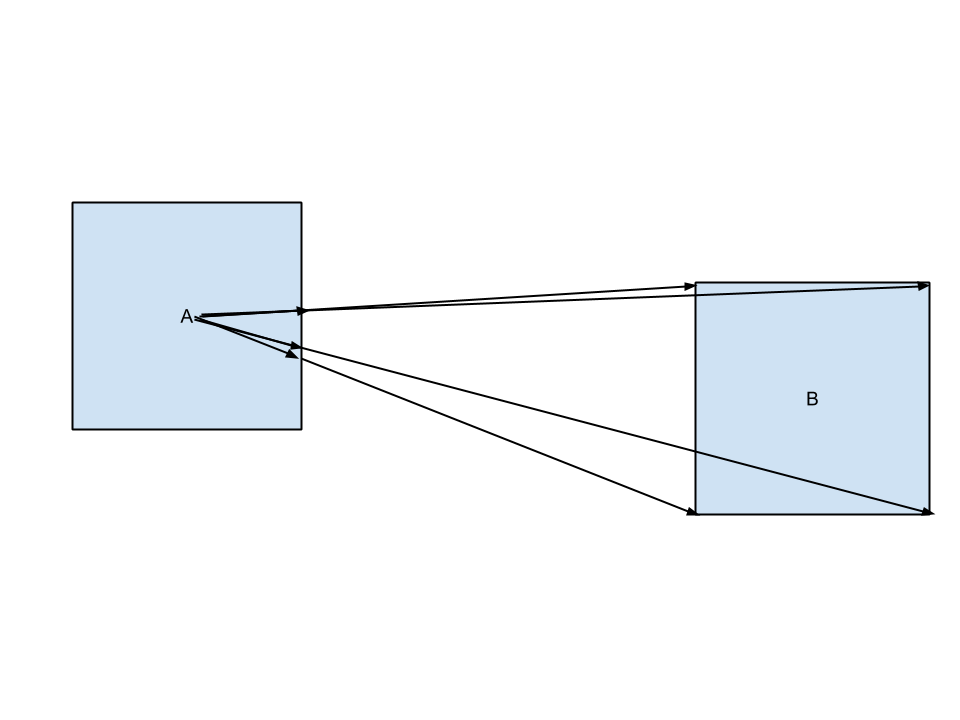
\includegraphics[width=0.48\textwidth]{figures/vision5.png}
	\end{center}
	\caption{The second iteration of the \texttt{canSee(A,B)} algorithm}
	\label{fig:vision5}
\end{figure}

This model was not perfect, however, in that it could give bias to a section of an object if there were a large number of vertices concentrated at a given section. In figure \ref{fig:vision6}, we show how this could be problematic. In this example, A would cast a disproportionate amount of rays to B's bottom side, which would collide with C, giving the impression that B is much less visible than it actually is.

\begin{figure}[h]
	\begin{center}
		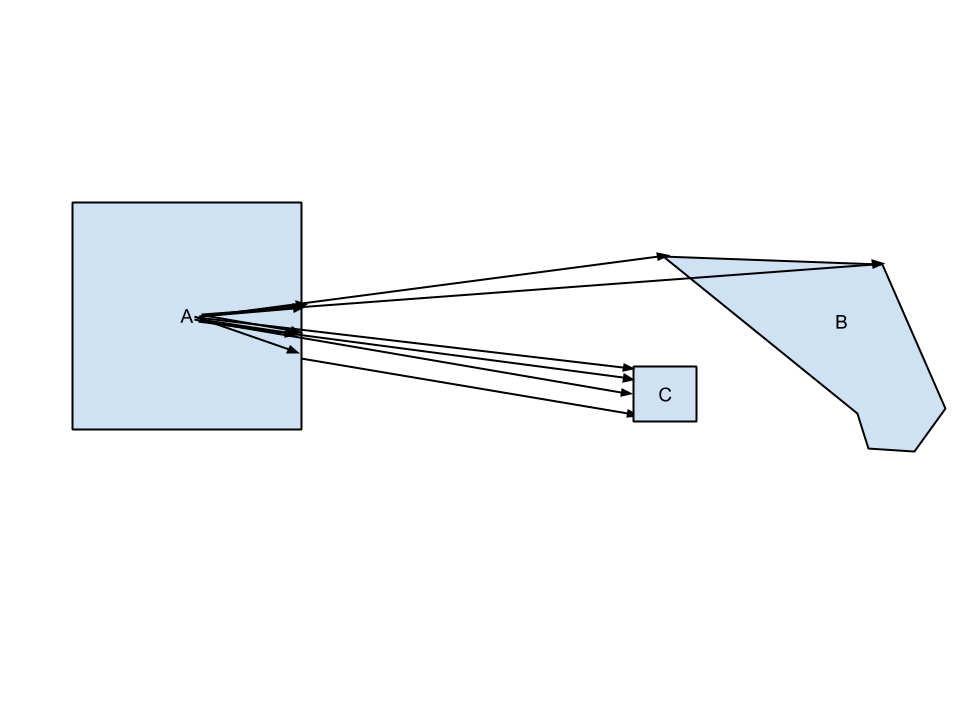
\includegraphics[width=0.48\textwidth]{figures/vision6.png}
	\end{center}
	\caption{The majority of the casts are blocked by C even though B is visible.}
	\label{fig:vision6}
\end{figure}

One suggested solution to this situation involved weighting the vertices depending on how close they were. In this interpretation, casts to close-by vertices would be “worth less.” If these successfully hit their target, they would return a number less than one. The exact weighting system was not decided. This system, however, proved to be unnecessary, as the final algorithm removed the need for vertices entirely. 

The final system utilized an obscure library in Blender Python (\texttt{BPY\_extras}) to grasp random points on the meshes faces. Rays were cast to these points, and the percent of casts that returned were used to evaluate the visibility of the target object. This method was both fair and correct. The number of rays cast to a given face was proportional to the face's percent of the total surface area of the object, which ensured that the most visible (largest) faces would receive the most casts. Because the number of samples is proportional to the size of the object's faces, no section of the object will over represent itself in testing. Figure \ref{fig:vision7} shows how the new method solves the problems of the old.

\begin{figure}[h]
	\begin{center}
		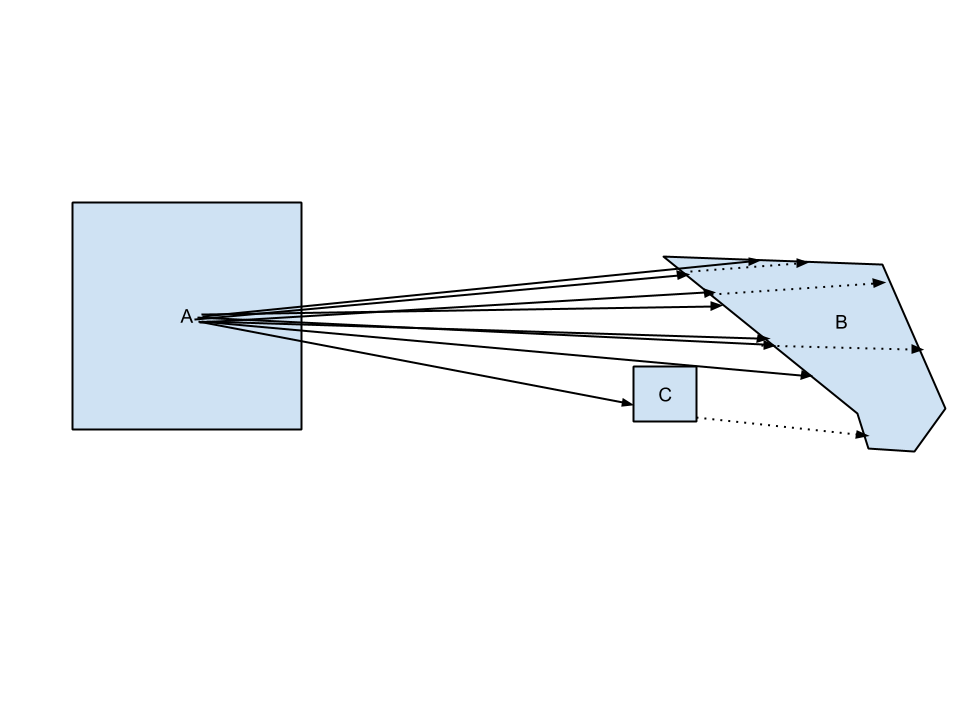
\includegraphics[width=0.48\textwidth]{figures/vision7.png}
	\end{center}
	\caption{Rays are cast evenly across object B.}
	\label{fig:vision7}
\end{figure}

The final change to the vision predication involved compensation for opacity. It was desired that the visibility of an entity not simply depend on line of sight, but also on the presence of partially occluding objects passed through en route to the goal object. This was solved through custom properties and repeated casting. Each ray-cast was given an initial value of 1. The cast traveled through space as in the above model. When another object was encountered, the behavior of the cast differed depending on the object hit. If the object was the target object, then the cast returned it's value (initially set to one). If it encountered a different object with no occlusion property (or an occlusion value of one) then the hit object was assumed to be completely opaque and the cast returned zero. A completely opaque object (one that would cause any ray to return 0 if it made contact), was specified with an occlusion of -1. If the object hit an object with an occlusion value between zero and one, then the object recast towards its target, but the value of the occlusion property was added to an “occlusion counter” for the cast. This occlusion counter would would be reduced by the occlusion amount of the object when the cast left the object.	

As the cast traveled through an object, the value would degrade proportional to the current counter. If the return value was reduced to zero, then the cast would fail and the function would return zero. Thus, the further through an obscuring object (such as a fog or the leaves of a tree) an object was, the more obscured it became. The “occlusion counter” was necessary in order to allow multiple obscuring factors affect the object. This corresponds to situations such as man looking at a bird through a tree in a fog.

The addition of occlusion necessitated the introduction of a new function in \texttt{obutily.py}: \texttt{cast\_thru}. This function performed all of the above functions, and took care of the repeated casting (including calls to ray\_cast and nudge). The initial cast was handled by the \texttt{predicateMethods.py} file, and subsequent casts were all done in the \texttt{cast\_thru method}. This led \texttt{canSee} to a slightly different larger dependence on \texttt{obutily.py} functions than other predications.


Originally, the starting point for \texttt{canSee} was the location of the first object in the predication.
Typically, this was the lowest point in the object, in the center of the xy plane. 
This presents an obvious issue for calculating visibility: human beings do not see with their feet. 
Thus, for models which were capable of vision, an additional ``eye'' was added to list of meshes. 
The \texttt{canSee} function was changed to begin ray tracing from the location of the eye, which was located just in front of the face of the figures. 

\subsection{Placement Methods}

\texttt{Place()} returns the areas in the Blender scene where the predicate holds for one entity relative to the other. This makes the assumption that the second object has already been placed; for example in the predication ``near(A,B)'', if \texttt{Place(A)} was called, it would return an acceptance area of ``nearness'' for A, such that the predication is satisfied. 
At present, the placement locations are returned as a tuple of pairs, with each pair containing the minimum and maximum values for the x, y, and z dimensions. This was meant to build of previous (similar) methods in Wordseye and Soar, which used similar methodology. \cite{wordseye,wintermute2009overview}.
The placement functions went through several iterations and different ideas, and were the subject of much revision over the course of the project.
For the first build of the project, the current system was implemented. Figure \ref{fig:square_placement} provides a visualization for this method.
 
\begin{figure}[h]
	\begin{center}
		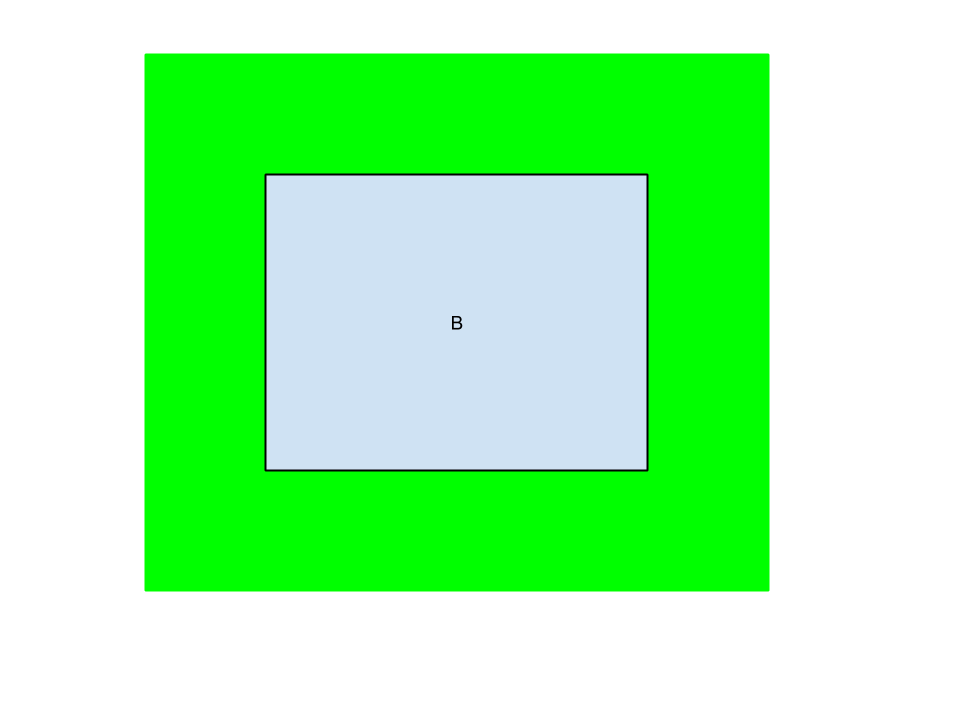
\includegraphics[width=0.48\textwidth]{figures/square_placement.png}
	\vspace{-1cm}
	\caption{A visualization of the first and current placement mechanism.}
	\label{fig:square_placement}
	\end{center}
\end{figure}

This system suffices for many predicates; however, it is not easily extensible to predications which have disjoint or disconnected valid placement areas. 
As such, there were concerns about whether a better placement paradigm was necessary.
In particular, the vision predicates can generate placement areas of this sort. Figure \ref{fig:vision_placement_theoretical} illustrates the issues that the system raised.

\begin{figure}[h]
	\begin{center}
		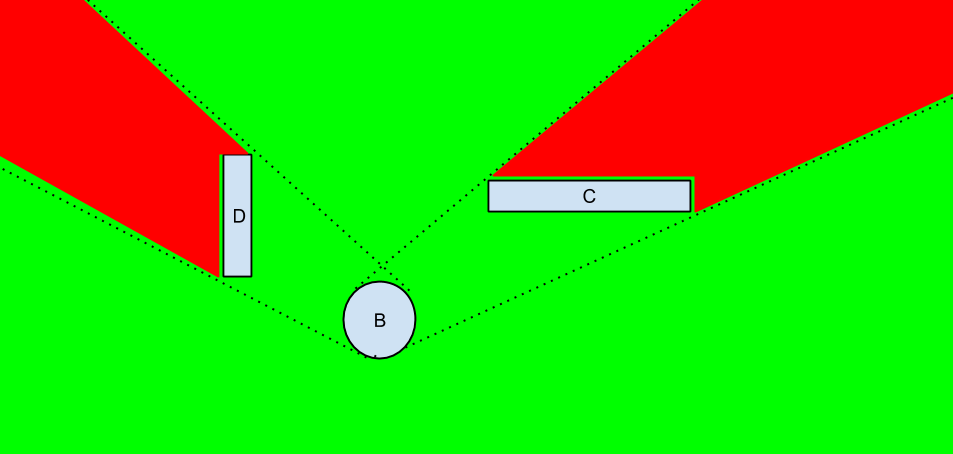
\includegraphics[width=0.48\textwidth]{figures/vision_placement_theoretical.png}
	\caption{The theoretical placement areas for the predicate \texttt{canSee}. Valid areas are colored green, invalid areas are red.}
	\label{fig:vision_placement_theoretical}
	\end{center}
\end{figure}

Several solution have been researched and proposed. Wordseye utilizes a the concept of ``valid placement polygons.'' 
This concept represents the valid placement areas of objects as polygons, and, with this heuristic, is able to choose the best area for inserting an object in a scene \cite{wordseye}. 
Another similar solution is proposed in Xu et al, where Minkowsky sums are utilized. This technique has been shown to be efficient in certain special cases of polygons, and was able to produce fruitful results in experimental trials \cite{xu2002constraint}. 

In this vein, I proposed the idea of utilizing multiple of our current placement rectangular-prisms (and their combinations) in order to represent the valid placement areas of a given polygon. 
This idea has been worked on and refined this idea into several possible solutions. One solution is the idea of the ``grid-box technique.'' 
In this technique, the geometry of placement areas is represented as an assembly of discrete 'boxes', one of which is sampled for a valid placement location of the given object.
Each box is represented a 3-tuple of pairs, corresponding to x, y, and z coordinates of a cube in three-dimensional space. 
These boxes, unlike their counterparts in the current placement system, are of a discrete and unchanging size, and are arranged in a tessellating fashion similar to a grid. 
In this method, a square is considered a valid placement area if all of it's points satisfy a the respective predication. Figure \ref{fig:grid_placement} below provides an illustration.

\begin{figure}[h]
	\begin{center}
		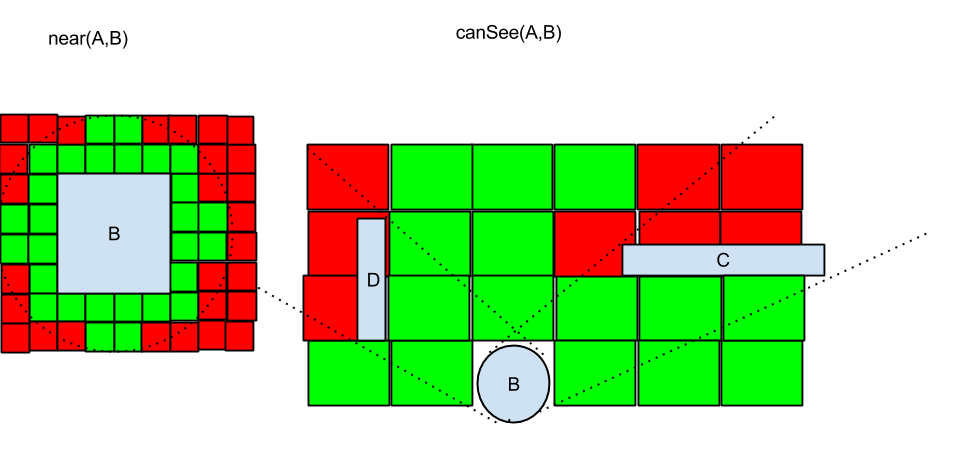
\includegraphics[width=0.48\textwidth]{figures/grid_placement.png}
	\caption{One proposed method of placing objects using by using a uniform grid of placement areas.}
	\label{fig:grid_placement}
	\end{center}
\end{figure}

Another proposed method is the rejection-sampling model. 
A short mockup of it was even built earlier this year. 
This model randomly selects points given a heuristic for the model, and rejects them if they fails to satisfy the specified predication or predications. 
\ref{fig:rejection_sampling_placement} below illustrates the system.

As previously noted, this system does allow for a very simple implementation (forgoing the placement prism entirely), though because it rejects so many potential points, The feasibility of this algorithm was a subject of investigation. 

A combination of rejection sampling and the standard ``block placement'' algorithm was used. The collective blocks of all the predications of an object are overlayed, their intersection being the new legal placement area. Rejection sampling is then used to sample locations from this space. The resulting configuration is queried. If all the predications are satisfied, the next object is placed. If it is not, then another spot is sampled, and the process begins again.

\begin{figure}[h]
	\begin{center}
		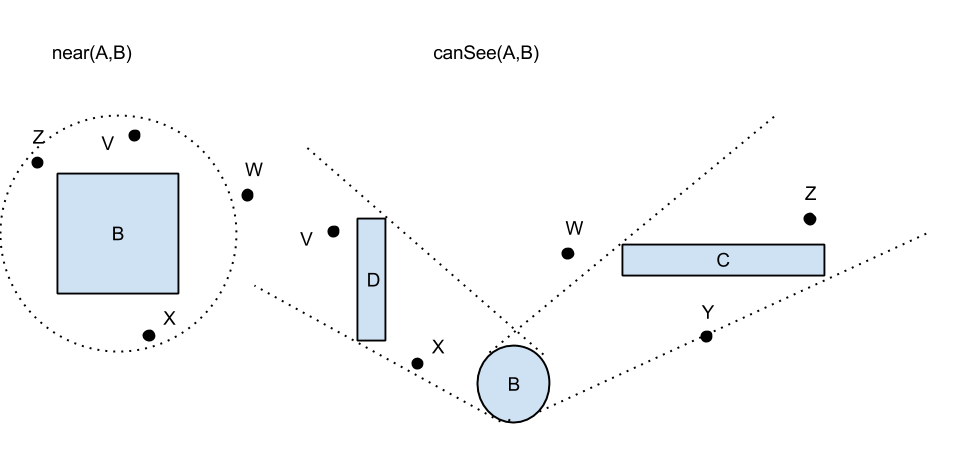
\includegraphics[width=0.48\textwidth]{figures/rejection_sampling_placement.png}
	\caption{Rejection sampling was also considered as a placement mechanism.}
	\label{fig:rejection_sampling_placement}
	\end{center}
\end{figure}      

\include{using-classes}    

\include{learning-classes} 

\include{using-ontology}   

\include{topic-models}     

As shown in figure \ref{table:query_results}, the system is able to handle the simple case for object querying very reasonably. 
The fastest calculating predicate is \texttt{isTouching}, followed closely by \texttt{near}.
Because these two predicates operate on similar algorithms, it make sense that the two operate in similar time.
One potential significance is the fact that \texttt{isTouching} operates faster than \texttt{near}, and the only tangible difference between the two algorithms is the fact that \texttt{isTouching} has a smaller threshold than \texttt{near}.
It was first speculated that this meant that the internal Blender functions relied on by these predication functions' run-time increased with object distance.
However, the more likely explanation is the calculation of the threshold between the two functions.
In \texttt{near}, the threshold is calculated with a function that operates in linear time.
In \texttt{isTouching}, it is a constant, predetermined value, and thus requires no overhead to calculate.

The program worked into the Cornell Cup's Haptek team, where it was used to simulate a person navigating a virtual maze.  
This project set out to equip a room with several Kinect cameras which monitored the movement of a person in the room. A program, receiving input from the cameras, would build a virtual maze in a virtual representation of the room. The person's virtual avatar would be inserted into this simulation. 

The person's motion would be tracked with the cameras, and the avatar would move with the user. If the avatar came into contact with one of the virtual walls in the maze, then a buzzing feedback mechanism would be triggered. This allows the user to navigate a virtual maze. Because this is a simulation in 3D space, the project utilized many of the aspects of the \TDS project, including several of the predicates, the models for ``person'' and ``wall,'' and the temporal updating feature of the 3D scene.

In a similar note, the use of Blender has opened up a number of options for future endeavors. Because Blender is a widely-used program with a broad range of applications and widespread compatibility, \TDS has the potential to be utilized in any number of studies and situations. For example, many 3D printers currently accept model input in file formats supported by Blender. At this year's Rochack Hackathon, we were able to 3D print one of the models. This model can be seen in figure \ref{fig:3D_Print}.

\begin{figure}[h]
	\begin{center}
		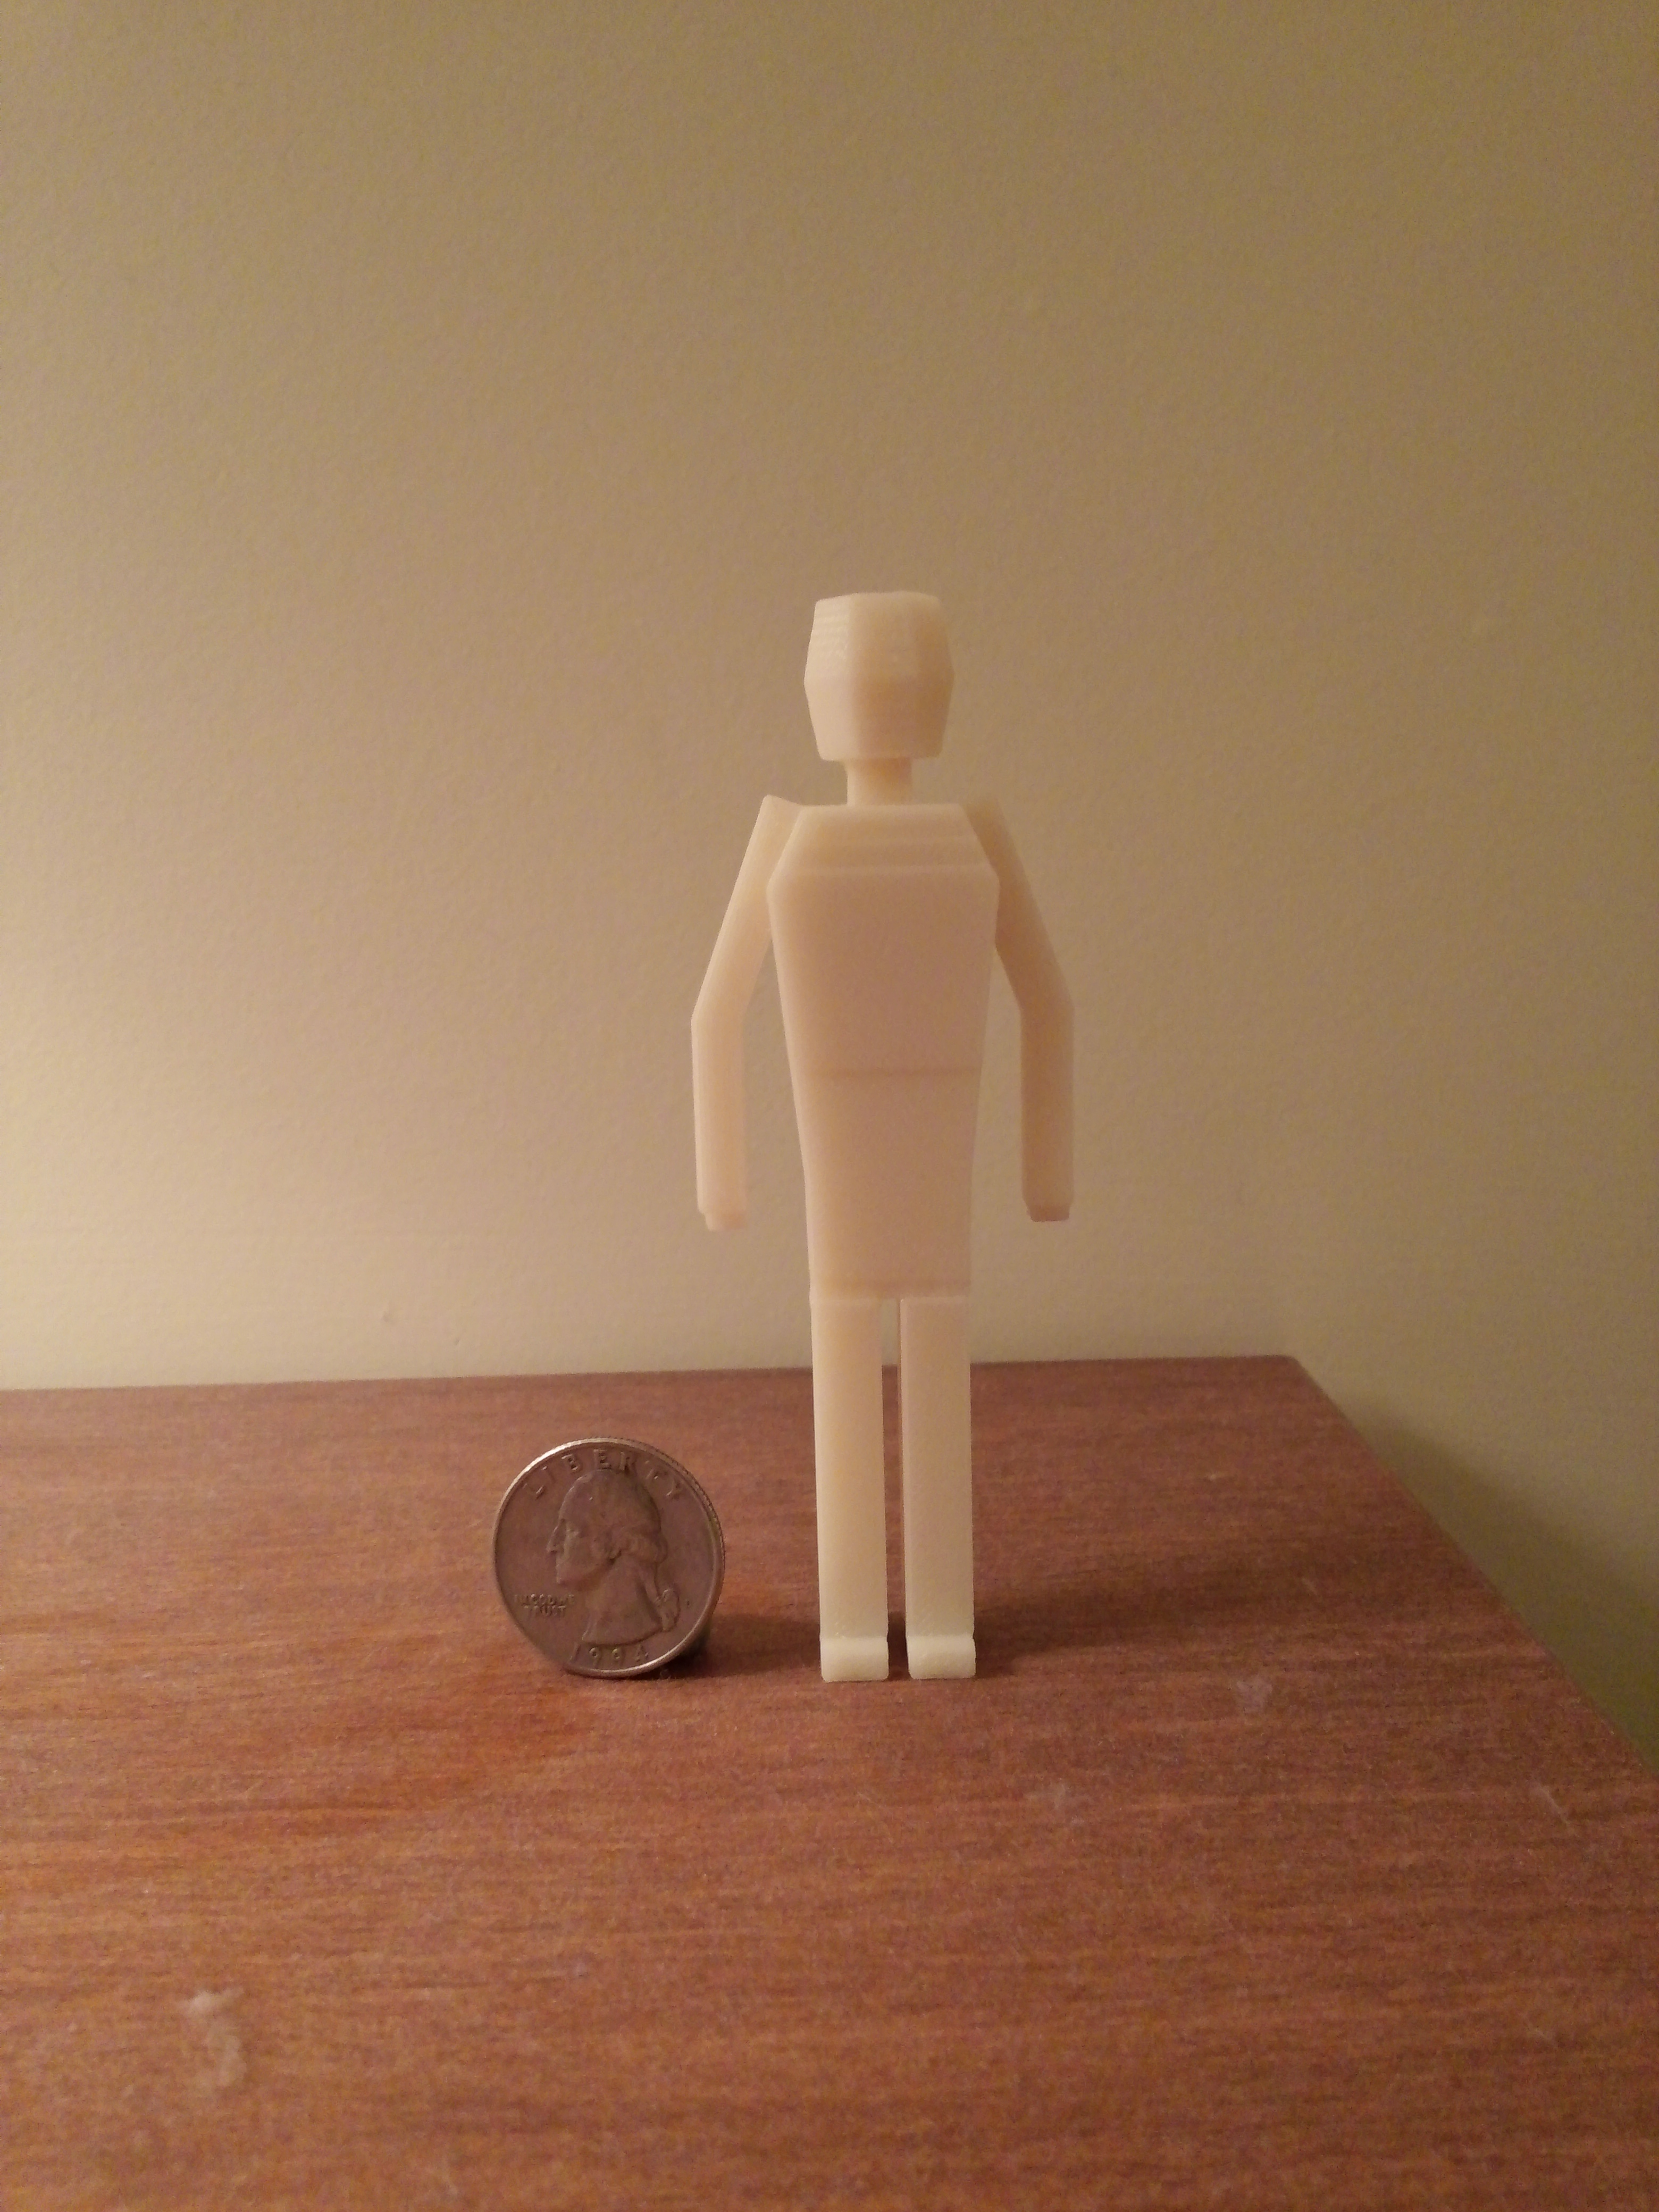
\includegraphics[width=0.45\textwidth]{figures/3D_Print.jpg}
	\end{center}
	\caption{The 3D printed model of the person from the story scene. A quarter is shown nearby for scale}
	\label{fig:3D_Print}
\end{figure} 

The Blender file for the person was uploaded with minimal changes to the 3D printer at the school, and printed. The entire process of converting the file, uploading it to the printer, and printing the figure took less than an hour. Given the growing importance of 3D printing in the present, and the many applications to 3D environments that \TDS offers, the ability to quickly model objects that can be 3D printed could prove to be a valuable feature of the system.

An area of concern is the run-time of the ``inside'' predication.
The run-time of this predication is significantly worse than the others. Because this function runs in $O(n^2)$ time, it is most likely not due to an inefficient algorithm. Rather, this lack of satisfiability is likely related to the legal placement area generated by the placement function in predMethods.py.

Inside is similar to in, differing only in that it requires one object to be inside the mesh (rather than bounding box) of the other. The legal area, however, is generated to encompass the entire bounding box. As such, it may overestimates the legal area by a considerable amount. Shrinking the placement area would potentially solve this problem, though it may prevent placement in legal areas. 

Our project was able to successfully query and place entities under predicate constraints. Because the scene was able to pass the original test of constructing the story-based image and deduce the implicit, spatial information in the scene (the person could not see the egg in the nest), the study was a success. The efficacy of rejection sampling in the placement function requires further investigation. Current testing indicates that it improves scene construction by making placements more accurate, though the key issue in this endeavor is the efficiency of the inside predicate.

The placement system creates a complex relationship between predications and entities during placement. An ``optimal'' order of placement emerges in complex scenes. Deviation from the optimal layout was shown to increase placement time dramatically.

The ``optimal'' configuration is one in which the entities are placed in order of decreasing number of predication constraints. For example, in the placement of the story scene, the required predications are:
\begin{center}
	\begin{itemize}
		\item a person is under a tree
		\item a nest is in a tree
		\item an egg is in the nest
		\item the person can see the nest
	\end{itemize}
\end{center} 
In this scene, the nest is the most constrained object, because it is used in a predication with the person (can see), the egg (in), and the tree (in). The least constrained entities are the tree and the person, each involved in only one predication. This forms a ``constraint hierarchy.'' 

For an optimal placement run-time, the entities in the scene should be placed from the most to least constrained. Placing the most constrained entities first allows the most legal placement area for the subsequent entities (which, because they are lower in the hierarchy, have naturally less constrained placement areas), which means that the system has to do less sampling and backtracking on average in order to place them.
Note that a constraint hierarchy is not necessarily unique for a given scene because multiple entities can be involved in the same number of predications.

The greatest flaw in the system, and the biggest boundary to continued expansion of the project, is the ad-hoc nature of the predicate and object database. 
Both entities and predicates are created in an ad-hoc fashion; there exist no templates for either, although some share similar features. 
Because of this, adding new members to either library can be cumbersome. 
Further, because the predicate functions of each are based on qualitative semantic interpretations of the predicates, it can be quite difficult to write functions that objectively represent the predicates they are meant to.

Our project's success in creating and querying 3D scenes demonstrates both its usability as a situation for reasoning in 3D spaces, and the expressive power of the system in general. 
Our program was able to quickly and efficiently manage and query over a small library of entities and predicates. 
The system is black-boxed to outside input, and as such can be used for more than just Epilog. Preliminary work with the 3D printed model and the collaboration with Haptek has shown this. The system, in its current form, holds potential to be of use in a number of projects and experiments that involve 3D space. We hope that the \TDS will be put to use as a specialist program, both in Epilog and beyond.

\bibliographystyle{named}
\bibliography{references}

\appendix
\include{generics}


\end{document}



